% supplement.tex — Physica A submission supplementary material, elsarticle
\documentclass[preprint,12pt]{elsarticle}

\usepackage{graphicx}
\graphicspath{{figures/}}
\usepackage{amsmath,amssymb}
\usepackage{bm}
\usepackage{hyperref}
\usepackage{xcolor}
\usepackage{booktabs}

\newcommand{\rb}{\rho_b}
\newcommand{\mc}{\mu_\mathrm{c}}
\newcommand{\kavg}{\langle k \rangle}
\newcommand{\Lsys}{L}
\newcommand{\rmin}{r_{\min}}
\newcommand{\kmax}{k_{\max}}

% S-prefix figure/section numbering, common supplement convention
\renewcommand{\thesection}{S\arabic{section}}
\renewcommand{\thefigure}{S\arabic{figure}}
\renewcommand{\thetable}{S\arabic{table}}
\renewcommand{\theequation}{S\arabic{equation}}

\journal{Physica A}

\begin{document}

\begin{frontmatter}

\title{Supplementary Material: \\
Adaptive rewiring produces sharp finite-size
bimodality in a conviction-weighted competitive network}

\author{Evan W. Martin}
\affiliation{Independent researcher}

\end{frontmatter}

% ══════════════════════════════════════════════════════════════════════════════
\section{Binder data-collapse details}
\label{sec:supp_collapse}

If the transition is asymptotically continuous, the
Binder curves should collapse onto a single master
curve under the standard finite-size scaling form
\begin{equation}
U_\Lsys(\mu) = \tilde{U}\!\left((\mu - \mc)\, \Lsys^{1/\nu}\right),
\label{eq:supp_collapse}
\end{equation}
with two free parameters~$\mc$ and $1/\nu$.
We attempt this collapse by minimising the per-point
inter-curve standard deviation of $U_\Lsys$ on a common
grid of the scaling variable $(\mu-\mc)\Lsys^{1/\nu}$,
restricted to the dip region $|\mu - \mc| \leq 0.012$
(outside this window all curves trivially asymptote
to $2/3$).
$\Lsys = 64$ is excluded from the fit: its anomalously
deep negative dip on a system of only $4096$~nodes is a
small-system fluctuation effect that no two-parameter
rescaling can absorb.

The three-size fit $\Lsys \in \{128, 256, 384\}$ does
\emph{not} collapse cleanly
(Fig.~\ref{fig:supp_collapse}, middle panel):
the $\Lsys = 128$ dip is much deeper than any rescaling
allows, leaving residual scatter
$\sigma_U \approx 0.04$.
Restricting to the two largest sizes
$\Lsys \in \{256, 384\}$ tightens the collapse by an order
of magnitude, $\sigma_U \approx 0.005$.
Bootstrap 95\% confidence intervals from 200
seed-resamplings give $\mc \in [0.346, 0.348]$ and
$1/\nu \in [0.97, 1.99]$.
The point estimate $1/\nu \approx 1.55$ should not be
over-interpreted: two curves fitted with two free
parameters provide a weakly constrained fit, and the
$1/\nu$ confidence interval spans most plausible
two-dimensional continuous-transition exponents.
The collapse therefore confirms only that
$\Lsys = 256$ and $\Lsys = 384$ are mutually consistent
with a standard FSS form, not a specific universality
class.

The contrast between the failed three-size and
acceptable two-size collapses is consistent with the
standard corrections-to-scaling picture of an approach
to a continuous transition: $\Lsys = 128$ lies outside
the regime where the leading-order finite-size scaling
form holds; $\Lsys \geq 256$ is more consistent with it.
Definitively settling whether the implied universality
class is robust would require either simulations at
$\Lsys \geq 512$ or systematic correction-to-scaling
fits with additional free parameters.

\begin{figure*}[t]
  \centering
  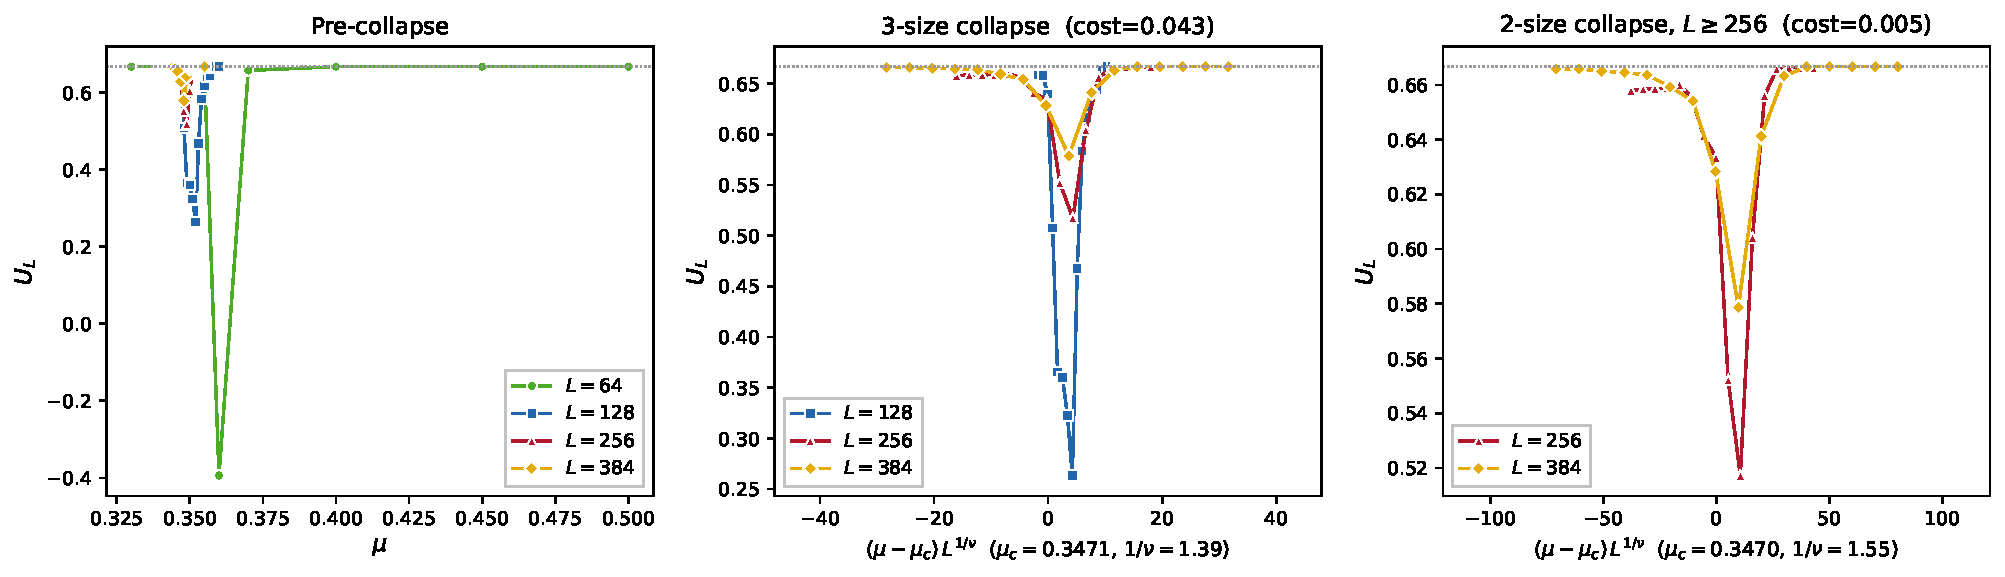
\includegraphics[width=\textwidth]{fig_data_collapse.pdf}
  \caption{%
    \textbf{Binder data-collapse attempt.}
    \textbf{Left:} raw $U_\Lsys$ vs.\ $\mu$ for all
    four sizes.
    \textbf{Middle:} collapse fit using
    $\Lsys \in \{128, 256, 384\}$;
    the $\Lsys = 128$ dip is much deeper than any
    two-parameter rescaling can absorb (mean inter-curve
    std~$\sigma_U \approx 0.04$).
    \textbf{Right:} restricting to the two largest sizes
    $\Lsys \in \{256, 384\}$ tightens the collapse to
    $\sigma_U \approx 0.005$.
    The contrast is consistent with $\Lsys = 128$ lying
    outside the regime where the leading-order
    finite-size scaling form holds.
  }
  \label{fig:supp_collapse}
\end{figure*}

% ══════════════════════════════════════════════════════════════════════════════
\section{Per-seed $\rb$ distributions at $\Lsys = 384$}
\label{sec:supp_hist_L384}

Figure~\ref{fig:supp_hist_L384} shows the per-seed $\rb$
distribution at $\Lsys = 384$ across the Binder minimum,
analogous to Figure~4 of the main text at $\Lsys = 128$.
At $\mu = 0.345$ the distribution is a tight unimodal
peak in the ordered phase ($\rb \approx 0.20$); at
$\mu = 0.351$ all 64 seeds have collapsed to a tight
unimodal peak in the disordered phase ($\rb \approx 0.55$).
Bimodality persists at the largest size, but only inside
a narrow window $\mu \in [0.347, 0.349]$ around the
Binder minimum---substantially narrower than the
$\Lsys = 128$ bimodal window.
The narrowing of the bimodal window with $\Lsys$ tracks
the same sharpening-yet-continuous trend as the Binder
recovery toward $2/3$ reported in the main text.

\begin{figure*}[t]
  \centering
  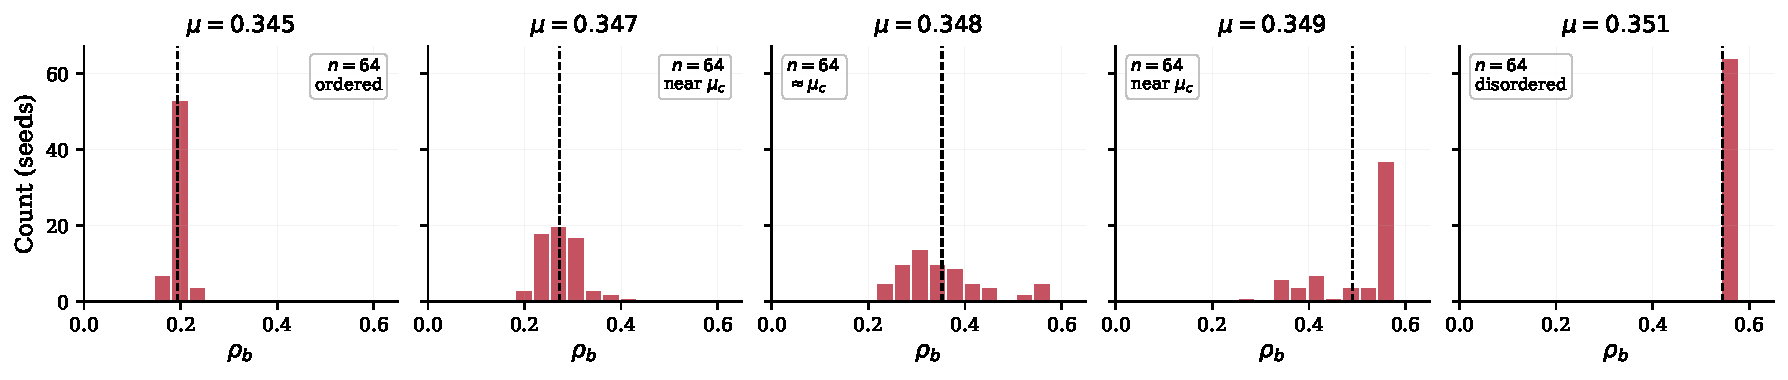
\includegraphics[width=\textwidth]{fig_hist_L384.pdf}
  \caption{%
    \textbf{Distribution of per-seed $\rb$ at
    $\Lsys = 384$ across the Binder minimum}
    (64 seeds per panel, 200\,000 frames).
    Bimodality persists at the largest system size but
    is confined to a narrow window
    $\mu \in [0.347, 0.349]$ around the Binder minimum
    ($\mc \approx 0.348$).
    Vertical dashed lines mark the mean.
  }
  \label{fig:supp_hist_L384}
\end{figure*}

% ══════════════════════════════════════════════════════════════════════════════
\section{Convergence diagnostics}
\label{sec:supp_convergence}

Figure~\ref{fig:supp_convergence} shows $\rb$
time-series for 8~seeds at three $\mu$ values at
$\Lsys = 256$ (snapshots every 5\,000 frames,
100\,000 total).
Away from the transition ($\mu = 0.341$ and $0.355$),
second-half averages are stable.
Near $\mc$ ($\mu = 0.349$), some seeds undergo
within-run phase switching, so reported second-half
averages for those seeds conflate the two basins.
Spot-checks at $\Lsys = 384$ (200\,000 frames) show
similar within-run basin-switching near $\mc$;
the doubled run length improves but does not eliminate
this near-critical residence-mixing effect.

\begin{figure}[t]
  \centering
  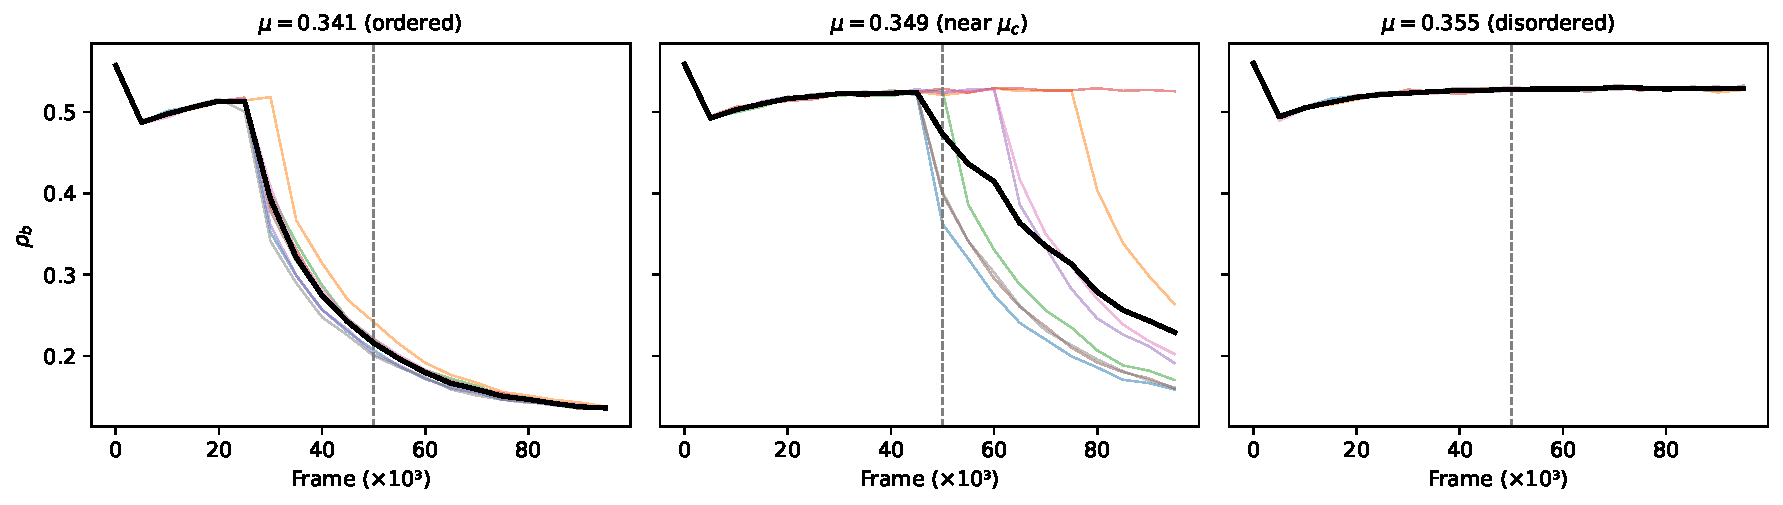
\includegraphics[width=\columnwidth]{fig_convergence.pdf}
  \caption{%
    \textbf{Convergence diagnostics at $\Lsys = 256$.}
    $\rb$ vs.\ frame for 8~seeds at three~$\mu$ values
    (snapshots every 5\,000 frames, 100\,000 total).
    Dashed line marks the burn-in cutoff (second-half
    averages are reported in the main text).
    At $\mu = 0.341$ (ordered) and $0.355$ (disordered),
    seeds converge within the burn-in window.
    At $\mu = 0.349$ (near~$\mc$), some seeds switch
    basins during the second half.
  }
  \label{fig:supp_convergence}
\end{figure}

\end{document}
